%
% TU/e Style Master Thesis template for LaTeX
%
% Public version 1.0
% 2010 - 2013 Thijs Nugteren and Joos Buijs
%
% THIS IS THE MAIN FILE (i.e. compile this file, compiling the others directly won't work)
%
\documentclass[a4paper,10pt,twoside]{report}

%all the other includes etc. are done in the thesis.sty file.
\usepackage{thesis}

%
% These commands need to be defined in order to produce a correct and personalized document
%
\newcommand{\shortdoctitle}{Seminar Report}
\newcommand{\doctitle}{Synthetic graph data generation}
\newcommand{\docsubtitle}{Web Engineering Seminar final report}

\newcommand{\me}{Thom Hurks}
\newcommand{\keywords}{gMark, graph generation, benchmarking}
\newcommand{\version}{0.1}
\newcommand{\monthYear}{January 2018}

%Be sure to use all the titles for your committee members!!! (their names show up on the very first page!)
\newcommand{\firstCommitteeMember}{dr. G.H.L. (George) Fletcher}
\newcommand{\secondCommitteeMember}{dr. N. (Nikolay) Yakovets}

\author{\me}

%
% PDF settings
%
\hypersetup
{
    pdfauthor={\me},
    pdftitle={\shortdoctitle},
    pdfsubject={\doctitle},
    pdfkeywords={\keywords}
}

\begin{document}

%use this include for PDF and distribution versions
\pagenumbering{roman}
\begin{titlepage}
\begin{center}

\includegraphics[height=2cm]{figures/tue-logo-high}\\
%\LARGE
%Eindhoven University of Technology \\
\large
Department of Mathematics and Computer Science  \\
Architecture of Information Systems Research Group

\vspace*{10cm}

\setlength{\TPHorizModule}{1mm}
\setlength{\TPVertModule}{\TPHorizModule}
% Set the Paragraph Indent to zero, so the first line is not Indented
% Back-up the current value so it can be put back at the end of the title page
\newlength{\backupparindent}
\setlength{\backupparindent}{\parindent}
\setlength{\parindent}{0mm}			
% Begins a textbox at 72 mm from the left of the edge of the paper and 89 mm from the top
% The width of the textbox is 95 mm (167 - 72 mm)
% The height of the box cannot be defined, so it is your task to keep the text not too long
\begin{textblock}{95}(62,89)
    \vspace*{1mm}
    \huge
    \textbf{\doctitle \\}
    \Large
    \vspace*{5mm}
    \textit{\docsubtitle}\\
    \vspace*{10mm}
    \Large
    \me\\
\end{textblock}

\large
Supervisors:\\
\begin{tabular}{rl}
    \firstCommitteeMember\\
    \secondCommitteeMember\\
    \thirdCommitteeMember\\
\end{tabular}

\vfill
\version

\vfill
%\docdate \\
\large
Eindhoven, \monthYear\\

% Put the Paragraph Indent back to its original value
\setlength{\parindent}{\backupparindent}
\end{center}
\end{titlepage} 

\normalsize

%Sometimes line numbers are nice, uncomment the next line to enable:
%\linenumbers

%It could be handy to have a list of todos and brainstorms in your thesis
%\chapter*{*General todos*}\todo{remove this chapter}
%\input{chapters/general_todos}

%\chapter*{*Brainstorm results*}\todo{remove this chapter}
%\input{chapters/brainstorm_results}

\chapter*{Abstract}\label{chapter:abstract}
The rise of social network applications over the past years has sparked massive interest in the study of such networks, specifically how to efficiently store and query them using databases. Besides that, many (social) domains are easily and naturally expressible in graphs and networks, such as corporate (financial) networks, criminal networks and even physical network systems such as the internet.

When studying social networks, or more general, graphs, it is obviously necessary to obtain test data. Such test data can be actual social networks or domain graphs, but this data is not always easily accessible. Companies and other institutions, such as governments, may have various reasons why they do not want to publish or share their graph databases. Reasons can vary from financial motivations where a company does not want to give away their core business asset to privacy concerns where data may not even be allowed to be shared. Sometimes the necessary graph data is available, but a researcher may require a much larger dataset to stress test a system, so additional data still needs to be obtained.

The solution to these problems is synthetic graph generation, where graphs with the appropriate size and structural properties are generated. These structural properties may be pre-defined using a graph schema or may be generated as well.
This report examines the state of the art regarding synthetic graph generation, specifically focusing on possible improvements or extensions that can be applied to gMark \cite{Bagan2016GMark:Queries}, a schema driven generator for graphs and associated query workloads.

%An executive summary if you want:
%\chapter*{Executive summary}\label{chapter:executive_summary}
%\input{chapters/executive_summary}

%\clearemptydoublepage


\chapter*{Preface}\label{chapter:preface}
Thanks go to dr. G.H.L. (George) Fletcher and dr. N. (Nikolay) Yakovets for their supervision over this project during the web engineering seminar.

\tableofcontents

%\listoffigures
%
%\clearemptydoublepage

%\listoftables
%
%\clearemptydoublepage

%\lstlistoflistings
%
%\clearemptydoublepage

\chapter{Introduction}\label{chapter:introduction}
\setcounter{page}{0}
\pagenumbering{arabic}
%from here on, start the 'real' page numbering, from 1, with normal digits
gMark \cite{Bagan2016GMark:Queries} is a domain- and query language-independent framework targeting highly tunable generation of both graph instances and graph query workloads based on user-defined schemas \cite{BaganG.andBonifatiA.andCiucanuR.andFletcherG.H.L.andLemayA.andAdvokaat2016GMarkProject}. As such, gMark can be used to generate synthetic graph instances to be used in experiments where graph datasets are needed but for various reasons not easily acquired. This study will first examine gMark's data model, then possible extensions to gMark's data model and will then examine the state of the art in the area of synthetic graph generation in order to identify possible improvements to gMark's graph generation capabilities.

%\chapter{Preliminaries}\label{chapter:preliminaries}
%\input{chapters/preliminaries}
%
%\clearemptydoublepage

\chapter{gMark data model}\label{chapter:gmark_definition}
gMark generates directed edge-labelled graphs \cite{Bagan2016GMark:Queries}. Edge-labeled graphs are graphs where labels are assigned to edges. These labels indicate the type of relationship that the edge denotes in the application domain.

\begin{defn}
The definition of an edge-labelled graph \cite{2017ADatabases}
    \begin{enumerate}
      \item $V$ is a finite set of vertices (or nodes).
      \item $E$ is a finite set of edges; formally, $E \subseteq V \times Lab \times V$ where $Lab$ is a set of labels.
    \end{enumerate}
    \label{def:edge_labelled_graph}
\end{defn}

Edge-labelled graphs are simple as they only consist of vertices, edges (relationships) and labels and as such widely used. For example, they form the basis of the Resource Description Framework (RDF) used for encoding machine-readable content on the world-wide web \cite{2017ADatabases}. In figure \ref{fig:edge_labelled_graph} you can see an example of an edge-labelled graph.

\begin{figure}[!ht]
    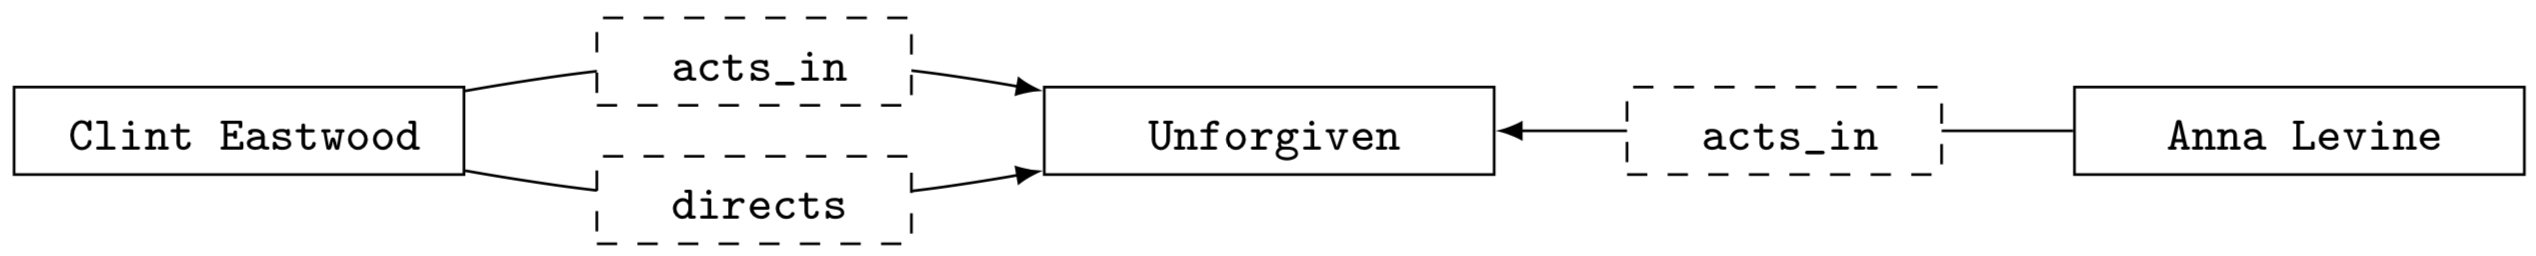
\includegraphics[width=\textwidth]{figures/edge_labelled_graph.png}
    \caption{An edge-labelled graph encoding basic movie information with dashed labels on edges\cite{2017ADatabases}}
    \label{fig:edge_labelled_graph}
\end{figure}

Since gMark generates directed edge-labelled graphs, we can amend definition \ref{def:edge_labelled_graph} by adding that a tuple $e \in E$ is ordered, and these edges may be called arrows or directed edges. For example, in a social network a directed edge $(A, knows, B)$ implies A knows B, but does not imply that B knows A.

Edge-labelled graphs do have limitations due to their simplicity. For example, it is not possible to label nodes. If you need to indicate what type a node is, you would need to create a new node with the name of the type and then create a directed "is" edge from the entity node to the type node. Various limitations of edge-labelled graphs can be worked around by simply creating more nodes and relationships to encode properties, but how does one encode that a person is born on a certain date? Creating nodes for every possible birthday and then creating "born on" relationships is certainly possible, but also very cumbersome and it greatly increases the size of the graph. It is also not possible to assign properties to the labelled edges, so if one wants to record properties of relationships such as the date the relationship is created, then that also requires more nodes and edges. Figure \ref{fig:edge_labelled_graph_downsides} shows a graph similar to the one in figure \ref{fig:edge_labelled_graph} but with extra nodes to encode various properties.

Another downside of edge-labelled graphs is that it is more difficult to indicate a schema. As per our example, a node for the person "Anna" may have an "is" relationship to the node "person" to indicate that Anna is a person. Anna may also have a "born on" relationship to the node "01-01-1988" to indicate she was born on that date. However, it is not clear in this way that being born on a certain date is in fact a property of being a person.

\begin{figure}
    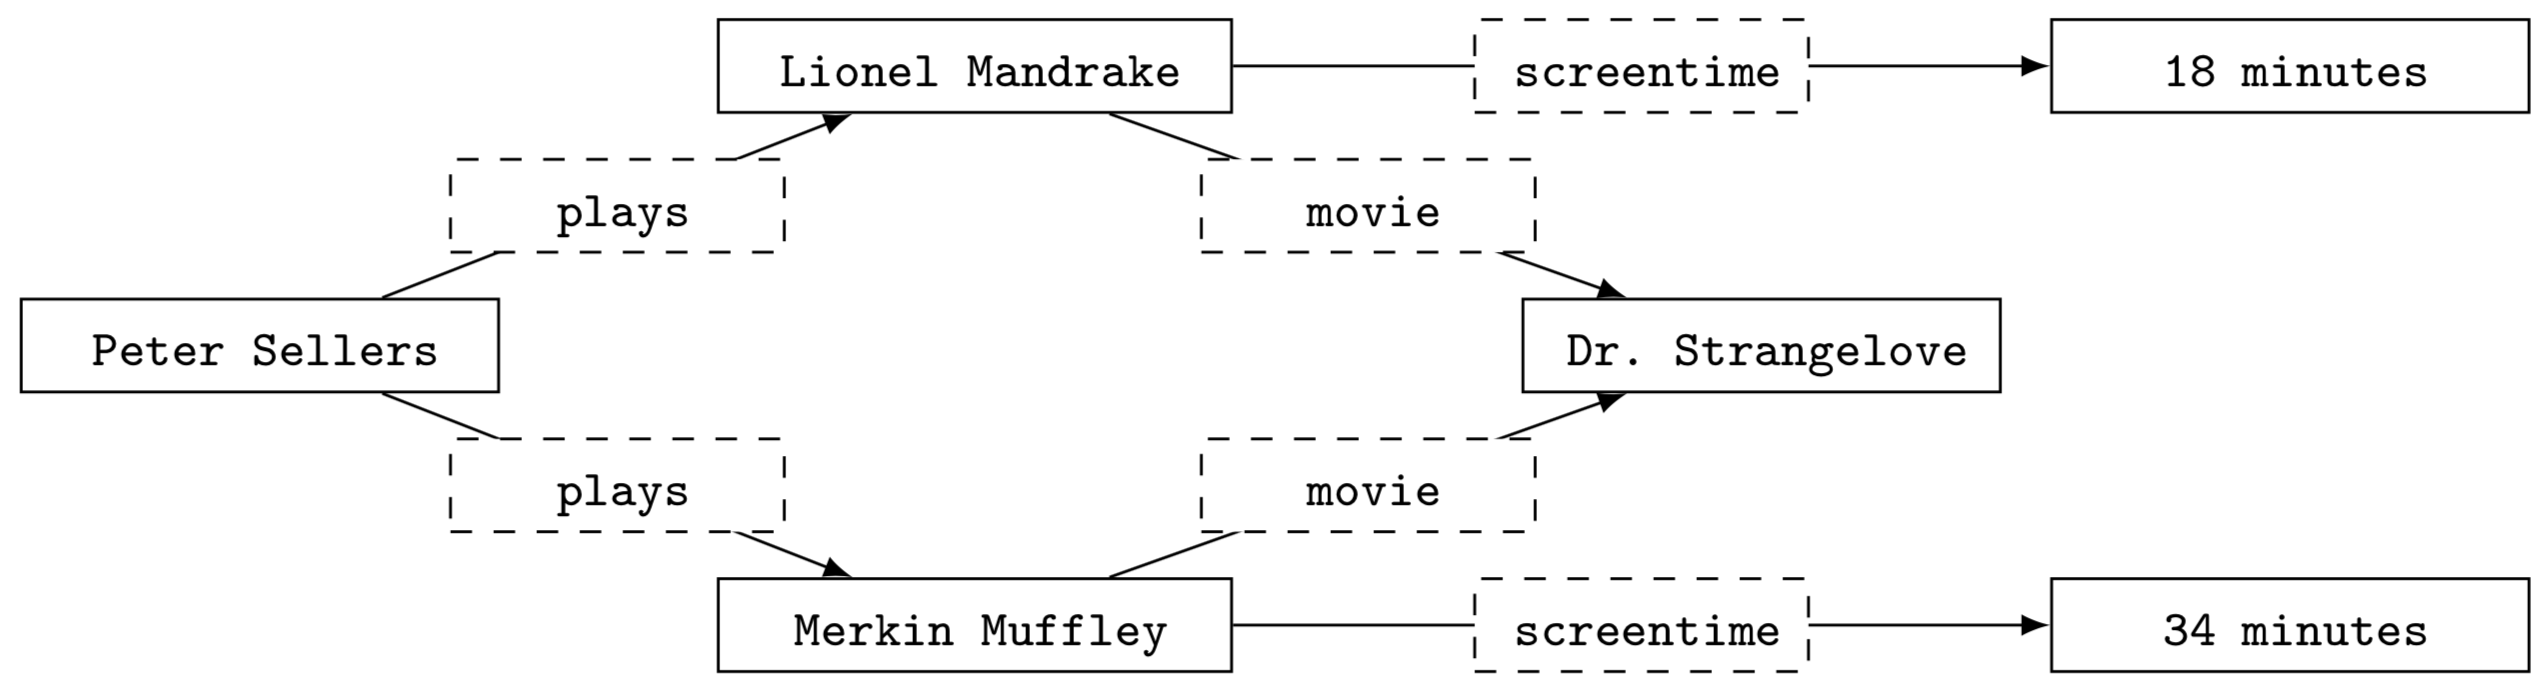
\includegraphics[width=\textwidth]{figures/edge_labelled_graph_downside.png}
    \caption{A version of figure \ref{fig:edge_labelled_graph} where extra nodes are used to encode properties \cite{2017ADatabases}}
    \label{fig:edge_labelled_graph_downsides}
\end{figure}

\chapter{Property graph data model}\label{chapter:property_definition}
To address the difficulties regarding edge-label graphs mentioned in the previous chapter, we can instead consider the property graph. Property graphs allow also labeling nodes, as shown in definition \ref{def:property_graph}. For example, in a social network one could have nodes of type Person and University. Whereas with edge-labeled graphs one would create a node Person and have a relationship "is" from nodes to the Person node to indicate those nodes are Persons, with property graphs we simply label those nodes as Person. Such a system makes the resulting graphs smaller and more intuitive to understand. In addition to labeled nodes, property graphs also associate attributes with edges and nodes. For example, a node of type Person can have the property \textit{family name}. Again, using extra nodes and edges this could also be modelled using an edge-labeled graph, but it would be more cumbersome. Also, with the property graph model we have a much more direct notion of a schema; the set of attribute names of nodes of a certain type can be considered as the schema of that node type. In edge-labeled graphs it is less clear which edges contribute to the schema of the node type and which edges express a relationship with a different node type, in addition to the fact that nodes cannot be labeled in edge-labeled graphs.

\begin{defn}
The definition of a property graph \cite{2017ADatabases}. A property graph $G$ is a tuple $(V, E, \rho, \lambda, \sigma)$, where:
    \begin{enumerate}
      \item $V$ is a finite set of vertices (or nodes).
      \item $E$ is a finite set of edges such that $V$ and $E$ have no elements in common.
      \item $\rho: E \rightarrow (V \times V)$ is a total function. Intuitively, $\rho(e) = (v_1, v_2)$ indicates that $e$ is a directed edge from node $v_1$ to node $v_2$ in $G$.
      \item $\lambda: (V \cup E) \rightarrow Lab$ is a total function with $Lab$ a set of labels. Intuitively, if $v \in V$ (resp., $e \in E$) and $\rho (v) = l$ (resp., $\rho (e) = l$), then $l$ is the label of node $v$ (resp., edge $e$) in $G$.
      \item $\sigma: (V \cup E) \times Prop \rightarrow Val$ is a partial function with $Prop$ a finite set of properties and $Val$ a set of values. Intuitively, if $v \in V$ (resp., $e \in E$), $p \in Prop$ and $\sigma (v,p) = s$ (resp., $\sigma (e,p) = s$), then $s$ is the value of property $p$ for node $v$ (resp., edge $e$) in the property graph $G$.
    \end{enumerate}
    \label{def:property_graph}
\end{defn}

By extending gMark to the property graph model, users can easily and clearly indicate different node types and give those nodes a set of attributes. For example, gMark could generate nodes of type Person each with attributes first name, family name, gender and birth date. This moves the scope of gMark away from just generating graphs and into the area of generating valid numeric and textual values for these attributes.

\chapter{Synthetic graph generation techniques}\label{chapter:graphgen_tech}
Before extending gMark, we examine the state-of-the-art in synthetic graph generation to see what other techniques exist and what the strengths and weaknesses of the various methods are.

\section{LDBC}
The LDBC (Linked Data Benchmark Council) uses a benchmark called the Social Network Benchmark \cite{Erling2015TheBenchmark, LDBCBenchmark}. To generate the scaleable synthetic data sets necessary for this benchmark, the LDBC uses a tool called datagen. The LDBC wants to use datasets with sensible PageRank outcomes and graph clustering structure, so their approach is to design a data model and generate data sets within this fixed model. Their data model has fixed node types such as "Person", "University", "Country" and the attributes of nodes of these types are generated using pre-defined functions (age) and dictionaries (name).
The advantage of using a fixed data model is that advanced correlations can be generated that would be difficult to generate in the generic case where nothing about the model is assumed. For example, datagen ensures that persons are more likely to be connected in the social network when they are similar. They accomplish this by pre-defining a similarity metric between nodes of type Person and by then grouping persons having similar scores together when generating edges. This ensures that persons living in the same location, studying at the same university or having similar interests are more likely to be connected in the network.
A few other correlations that datagen ensures are sensible are person name with respect to location and gender, person email address with respect to the popularity of the email's domain name, IP address with respect to location and duration of employment with respect to age.
The result is that datagen can generate graphs containing realistic data up to correlations between attribute values, but the clear downside is that it can only generate graphs with one specific fixed schema. Graphgen cannot generate graphs based on an arbitrary schema.

\section{Kronecker graphs}
Kronecker graphs are based around the Kronecker product. The Kronecker product is an operation on two matrices as shown in definition \ref{def:kronecker_product}.

\begin{defn}
    $A \otimes B =$
    \begin{bmatrix}
        a_{11}\textbf{B} \dots a_{1n}\textbf{B} \\
        \vdots \ddots \vdots \\
        a_{m1}\textbf{B} \dots a_{mn}\textbf{B}
    \end{bmatrix}
    for matrices A, B. \cite{Edu2010KroneckerLeskovec}
    \label{def:kronecker_product}
\end{defn}

The Kronecker product of two graphs is then the Kronecker product of their corresponding adjacency matrices \cite{Edu2010KroneckerLeskovec}. This can be used to generate synthetic graphs as follows. Firstly, take or randomly generate an initiator graph. Take the Kronecker product of this graph with itself to produce a new graph. One can then keep iteratively taking the Kronecker product of the resulting graph with itself in order to produce new bigger graphs.
The reasoning behind this process is to recursively create self-similar graphs that exhibit the densification power law, for which the Kronecker product is suitable. The recursive self-similar structure can be observed in figure \ref{fig:kronecker_matrix}. Intuitively, real-world communities also recursively create new communities, which is how Kronecker graphs mimic real-world social networks.

\begin{figure}[!ht]
    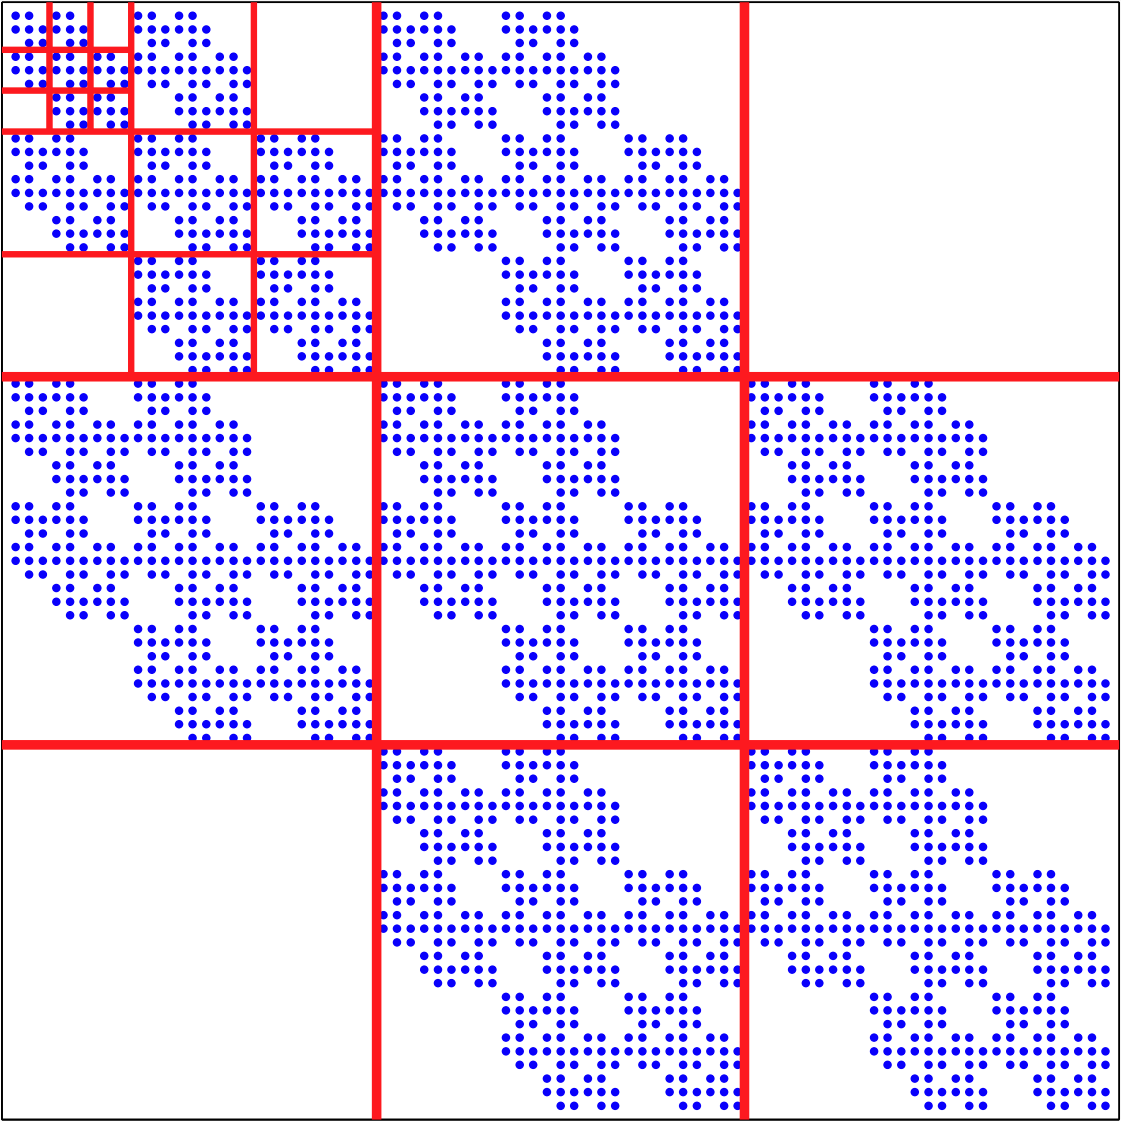
\includegraphics[width=0.5\textwidth]{figures/kronecker_adj_matrix.png}
    \caption{The adjacency matrix of the $4^{th}$ Kronecker power of a matrix. Dots are non-zero matrix entries, white space represents zeroes. \cite{Edu2010KroneckerLeskovec}}
    \label{fig:kronecker_matrix}
\end{figure}

By nature of their discrete creation process, Kronecker graphs exhibit a "staircase effect" in various metrics such as degree distribution and network value. The solution is to add randomness to the creation process to form stochastic Kronecker graphs. This variant works as follows. The adjacency matrix of the initiator graph now becomes a probability matrix. Each value $[0,1]$ denotes the probability that the edge is present. Apply the Kronecker graph creation process as usual. The end result then defines a probability distribution over all graphs. One can then simply sample an instance from this distribution.\cite{Edu2010KroneckerLeskovec}

As we are interested in generating synthetic graphs given a certain specification, the question now becomes how to tune the Kronecker creation process. Leskovec et al. \cite{Edu2010KroneckerLeskovec} describe an optimization process that aims to find an initiator matrix that has the highest likelihood to produce the adjacency matrix of a given real graph. The idea is that if the adjacency matrices of the synthetic graph and the real graph are similar then the global statistical properties over these graphs will also match. An implementation of this process called KronFit is available as open-source software as part of the Stanford Network Analysis Platform (SNAP). \cite{Leskovec2016SNAP:Library}

A clear advantage of Kronecker graphs is that one can generate graphs exhibiting desirable structural properties also found in real-world networks "from nothing" and that one can also generate synthetic graphs matching a given real-world graph by carefully choosing the initiator matrix. However, Kronecker graphs are not an all-in-one solution as they do not solve the problems of generating nodes of various types, generating different kinds of relationships and generating node attribute values. Assigning attribute values randomly to nodes would violate sensible correlations such as persons having friends within the same age group as themselves. Either one would need to graft labels, predicates and attribute values onto a Kronecker graph after-the-fact or the graph generation process somehow needs to account for attribute correlations and node type and predicate distributions.

\section{MAGs}
The multiplicative attribute graph (MAG) model is a stochastic network model that captures the interactions between node attributes and the network structure. \cite{Kim2012MultiplicativeNetworks} It only considers nodes with categorical attributes. In the MAG model, categorical node attributes have affinities to compute the probability of a link in the network. Affinities can be positive, such as shared interests increasing the probability of a link, or negative, such as same gender decreasing the probability of a relationship link. Formally, each categorical attribute has a square affinity matrix where the distinct categorical values form both the rows and the columns. Each cell of the matrix then stores the probability $p_{ij} \in (0,1)$ for a pair of nodes to form a link, given given attribute value $i$ of the first node and the value $j$ of the second node. The total link probability between two nodes is then the product of all the selected cells of the affinity matrices of the attributes of the nodes. The MAG model was proved \cite{Kim2012MultiplicativeNetworks} to capture patterns observed in real-world networks, such as power-law distributions, small diameters, unique giant connected component and local clustering of the edges.
Once a set of nodes with categorical attribute values is generated and a set of affinity matrices is constructed, the MAG model can be applied to generate the final graph. Affinity matrices can possible be manually constructed, but much more interesting and less tedious is to estimate the affinity matrices from a given graph. More specifically, given a network one wants to estimate the parameters of the distributions used to generate the node attribute values as well as the affinity matrices. An algorithm called MAGFit \cite{KimModelingModel} was developed with this purpose and is available as open-source software as part of the Stanford Network Analysis Platform (SNAP). \cite{Leskovec2016SNAP:Library} Unfortunately, MAGFit assumes that each node attribute takes the value $0$ or $1$ and follows a Bernoulli distribution, such that each affinity matrix is $2$ by $2$. This limits the applicability of the MAGFit algorithm in practice where synthetic graph nodes are expected to have realistic and usable values. Also, the MAG model does not tackle the problem of non-categorical node attributes.

\section{GScaler}
GScaler \cite{ZhangGSCALER:Graph} is a method for scaling an existing graph, analogous to DNA shotgun sequencing. GScaler works as follows. First, for each node in the input graph generate two pieces: a node with incoming edges and a node with outgoing edges. The result of this step is two bags (multisets) of pieces, one containing only pieces with incoming edges, and one containing only pieces with outgoing edges. Both bags are then scaled, ensuring the proportion of the pieces stays the same. After the scaling step it is possible the number of edges is incorrect, so the in- or out-degree of a few nodes can be adjusted in order to correct this. The pieces are then connected back to form nodes again, while making sure that the proportion of each node with a given combination of in- and out-degree stays the same. These nodes are then again connected together, ensuring that the proportion of the pairs of nodes $A$, $B$ where node $A$ has a certain in- and out-degree and node $B$ has a certain in- and out-degree stays the same. Once all nodes are connected back together, the result is a scaled graph. It must be noted that this whole process is never perfect; in each step a solution is chosen that is as optimal as possible, where the optimization is done using the Manhattan distance. GScaler produces graphs more similar to the original graph than a method like stochastic Kronecker graphs, but just like Kronecker graphs it only generates the graph structure and does not account for node attributes. Also, the GScaler algorithm does not account for graphs that have multiple node types and where relations may only be valid between nodes of certain types.

\section{DataSynth}


\chapter{Correlated attribute values}\label{chapter:correlated_attributes}
\input{chapters/attributes}

%\chapter{Conclusions}\label{chapter:conclusions}
%\input{chapters/conclusions}

%Choose a good bibliography style, plain would do often, but these might be nice too
%\bibliographystyle{these}
\bibliographystyle{plain}
\bibliography{mendeley}

%\clearemptydoublepage

%\appendix
%\addcontentsline{toc}{chapter}{Appendix}

%\chapter{My First Appendix}
\c

\end{document}
